


\documentclass[crop,tikz]{standalone}% 'crop' is the default for v1.0, before it was 'preview'
%\usetikzlibrary{...}% tikz package already loaded by 'tikz' option
\usetikzlibrary{trees}
\usetikzlibrary{shapes}
\usetikzlibrary{trees}
\usetikzlibrary{shapes}
\usetikzlibrary{matrix, fit}
\usetikzlibrary{arrows}
\usetikzlibrary{shapes}

\usepackage{bm}

\begin{document}



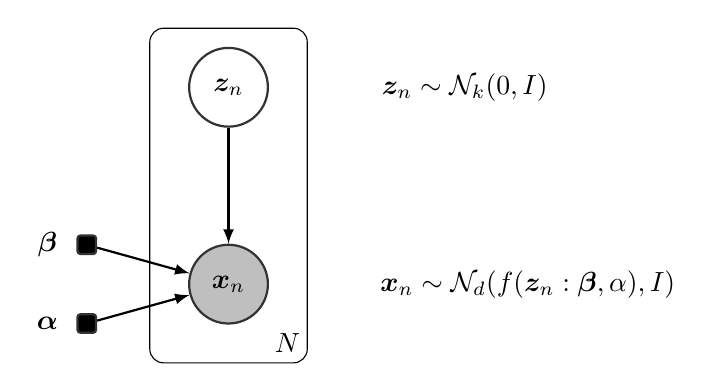
\begin{tikzpicture}

\tikzstyle{hidden}=[circle, minimum size = 10mm, thick, draw =black!80, node distance = 16mm]
\tikzstyle{observed}=[circle, minimum size = 10mm, thick, draw =black!80, node distance = 16mm, fill=gray!50]
\tikzstyle{trainvar}=[rectangle, minimum size = 2mm, rounded corners=1pt, thick, draw =black!80, node distance = 16mm, fill=black]


\tikzstyle{connect}=[-latex, thick]


\node[observed] (xn) at (0,-1)  {$\bm{x}_n$};
\node[hidden] (zn) at (0,1.5)  {$\bm{z}_n$};
\node[trainvar] (beta0) at (-1.8, -0.5)  {};
\node[trainvar] (alpha0) at (-1.8,-1.5)  {};

\node[] () at (-2.3, -0.5)  {$\bm{\beta}$};
\node[] () at (-2.3,-1.5)  {$\bm{\alpha}$};



\node (xd) at (3.8,-1)  {$\bm{x}_n \sim \mathcal{N}_d(f(\bm{z}_n : \bm{\beta}, \alpha),I) $};
\node (zd) at (3,1.5)  {$\bm{z}_n\sim \mathcal{N}_k (0,I)$};



%
%\node (betad) at (2.5,-2)  {$\bm{\beta} \sim \mathcal{N}_{d\times k}(0,I)$};
%\node (betad) at (4,-2)  {$\alpha \sim \mathcal{N}_{d\times k}(0,I)$};

\path (zn) [connect]  edge (xn);

\path (beta0) [connect]  edge (xn);
\path (alpha0) [connect]  edge (xn);



\draw[rounded corners=5pt]
  (-1,2.25) rectangle (1,-2);
  


%\path (det3) [connect]  edge (sum);


\node at (0.75,-1.75) {$N$};




\end{tikzpicture}
\end{document}